\documentclass[a4paper]{article}

%% Language and font encodings
\usepackage[english]{babel}
\usepackage[utf8x]{inputenc}
\usepackage[T1]{fontenc}
\usepackage{amsmath}
\newcommand\norm[1]{\left\lVert#1\right\rVert}

%% Sets page size and margins
\usepackage[a4paper,top=3cm,bottom=2cm,left=3cm,right=3cm,marginparwidth=1.75cm]{geometry}

%% Useful packages
%%%%%%%%% begin snippet
%% You need to add the package "tabularx".
%% Place the snippet right after \begin{document}

% need tabularx
\usepackage{tabularx}
\usepackage{amsmath}
\usepackage{graphicx}
\usepackage[colorinlistoftodos]{todonotes}
\usepackage{paralist}
\usepackage{amssymb,amsmath,amsthm,enumitem}
\usepackage[colorlinks=true, allcolors=blue]{hyperref}
\usepackage{subcaption}
\setlength{\abovedisplayskip}{3pt}
\setlength{\belowdisplayskip}{3pt}
\usepackage[hypcap=false]{caption}

\captionsetup{justification=centering}
\captionsetup{format=plain, font=small, labelfont=bf}

\begin{document}
\title{ Computational Intelligence, SS2018 Assignment 4}

\begin{titlepage}
       \begin{center}
             \begin{huge}
				   %% Update assignment number here
                   \textbf{Assignment 4}
             \end{huge}
       \end{center}

       \begin{center}
             \begin{large}
                   Computational Intelligence, SS2018
             \end{large}
       \end{center}

       \begin{center}
 \begin{tabularx}{\textwidth}{|>{\hsize=.33\hsize}X|>{\hsize=.33\hsize}X|>{\hsize=.33\hsize}X|} 

                   \hline
                   \multicolumn{3}{|c|}{\textbf{Team Members}} \\
                   \hline
                   STRUGER & Patrick & 01530664 \\
                   \hline
                   B\"OCK & Manfred & 01530598 \\
                   \hline
                   HAUPT & Anna & 01432018 \\
                   \hline

             \end{tabularx}
       \end{center}

\end{titlepage}

%%%%%%%%% end snippet

\newpage
\tableofcontents
\newpage

\section{Maximum Likelihood Estimation – BACKGROUND}

\begin{figure}[htp]
\centering
  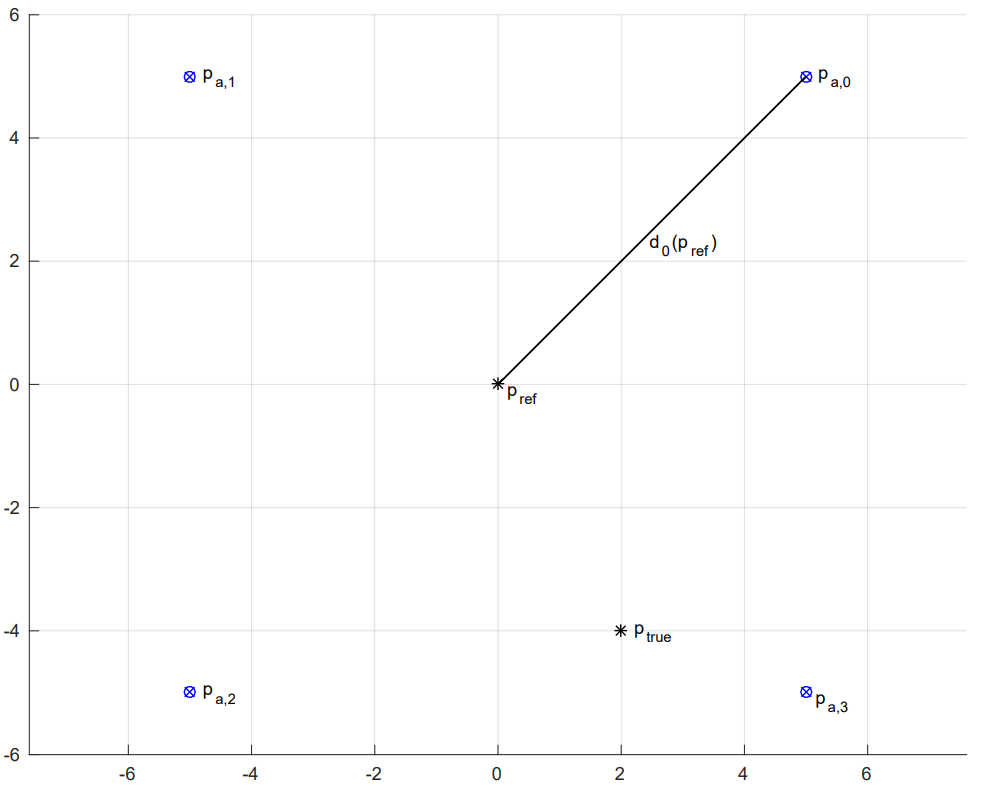
\includegraphics[scale=0.38]{plots/four_anchors.png}
  \captionof{figure}{ Four anchors (at known positions $p_{a,i}$, like the satellites in GPS) should be used to estimate the position of an agent, indicated as $p$. For calibrating the anchors we use $pref$.}
  \label{fig:15}
\end{figure}

\subsection{ Scenario and model}
The aim of this exercise is to estimate the position $p = [x, y]^T$ of an agent using (independent and identically distributed) noisy distance measurements $r_i, i = 0, . . . , N_A − 1$ to the $N_A = 4$ anchor nodes. These are shown in Fig. 1, and are at the positions

\[
P_{a,0}=
  \begin{bmatrix}
    5  \\
    5
  \end{bmatrix},
P_{a,1}=
  \begin{bmatrix}
    -5  \\
    5
  \end{bmatrix},
P_{a,2}=
  \begin{bmatrix}
    -5  \\
    -5
  \end{bmatrix},
P_{a,3}=
  \begin{bmatrix}
    5  \\
    -5
  \end{bmatrix}.
\]
We are not able to measure the \textit{true} distance $d_i(p)$ between the agent at position $p$ and the anchors. Hence, we need a statistical model that describes the error in the measurement $r_i$ and relates it to the unknown parameter $p$ that we want to estimate. We consider different cases, in which the distance measurements to the \textit{i}-th anchor are distributed as

\[
Case ~I ~(Gaussian): p(r_i|p) = \frac{1}{\sqrt[]{2\pi\sigma^2_i}}e^{-\frac{(r_i-d_i(p))^2}{2\sigma^2_i}}
\]
\[
Case ~2 ~(Exponential): p(r_i|p) = \begin{cases} \lambda_i e^{-\lambda_i(r_i-d_i(p)),} & r_i\geq d_i(p)\\ 0 & else  \end{cases}
\]

The dependence on the parameter $p$ is given as the Euclidean distance to the \textit{i}-th anchor, i.e.
\[
d_i(p) = \sqrt[]{(x_i-x)^2 + (y_i-y)^2}.
\]
Ideally we would like to obtain the ML estimation of the position $p$, i.e.,

\[
\hat{P}ML = arg ~\underset{p}{max} p(r|p) = arg ~\underset{p}{max} \prod_{i=1}^{N_A} p(r_i|p)
\]

The nonlinear dependence in (4), however, does not allow for a closed form solution of an ML estimator for $p$. A popular approximation to the maximum likelihood estimator is the least-squares estimator, i.e., to minimize the sum of squares of the measurement errors:
\[
\hat{P}ML \approx \hat{P}LS = arg ~\underset{p}{min} \sum_{i=1}^{N_A} (r_i-d_i(p))^2 = \norm{r-d(p)}^2 
\]

where the vector $r$ contains all $N_A = 4$ distance measurements $r_i$, and $d(p)$ is a vector that contains distances to all anchors $d_i(p)$, according to (4).
However, $d_i$ still has a nonlinear dependence of $p$. Therefore, we will use an iterative algorithm – the Gauss-Newton algorithm – to obtain the least-squares approximation: It requires the calculation of the Jacobian matrix of the measurement errors, which collects the first-order derivatives (linearizations) of the measurement errors. In this example, this matrix has the dimensions $(N_A × 2)$. The two columns are defined as

\[
[J_r(p)]_{i,1} = \frac{\partial(r_i-d_i(p))}{\partial x} \quad [J_r(p)]_{i,2} = \frac{\partial(r_i-d_i(p))}{\partial y}.
\]

The algorithm starts with an initial guess $\hat{P}^(0)$ and updates the parameter in the \textit{t}-th iteration as

\[
\hat{p^{(t+1)}} = \hat{p^{(t)}} - \Big ( J^T_d(\hat{P}^{(t)})J_d(\hat{P}^{(t)})\Big) ^{-1} J^T_d(\hat{P}^{(t)}) \Big (r-d(\hat{P}^{(t)}) \Big)
\]

The algorithm stops after a previously defined maximum number of iterations or if the change in the estimated position is smaller than a chosen tolerance value $ \gamma, i.e., \norm{\hat{P}^{(t)} - \hat{P}^{(t-1)}} < \gamma$.

\section{Maximum Likelihood Estimation of Model Parameters}

First we must specify the statistical model and estimate the according model parameters. In order to do so reference measurements were performed at a known distance $d_i(pref)$.
We use three different scenarios for the evaluation. Each scenario considers a different assignment of the measurement models (2) and (3):

\begin{itemize}[label={}]
  \item \textbf{Scenario 1:} Measurements of all anchors follow the Gaussian model.
  \item \textbf{Scenario 2:} Measurements of one anchor follow the Exponential model, the other ones follow the Gaussian model.
  \item \textbf{Scenario 3:} Measurements of all anchors follow the Exponential model.
\end{itemize}

Note that anchors with the same type of error-distribution also have the same parameters, i.e., the measurements are sampled from the same distribution.
The according measurements are contained in the files reference\_i.data as $(N × N_A)$ matrices $R$, where $N = 2000$ is the number of measurements.

\begin{itemize}[label={}]
  \item For scenario 2, find out which is the anchor with exponentially distributed measurements.
  \item Analytically derive the maximum likelihood solution for the exponential distribution.
  \item Estimate the parameters of the measurement models (2) and (3), i.e., estimate $\sigma^2_i$ and $\gamma_i$ for all anchors in all 3 scenarios using the maximum likelihood method.
\end{itemize}

\section{Estimation of the Position}
After specification of the statistical model we can estimate the position of the agent at an unkown position. Note that the estimation of the position must not take into account the true position but only the measurement data provided in measurements\_i.data . We further provide the true position \textbf{ptrue} for error evaluation.

\subsection{Least-Squares Estimation of the Position}
First, we will use the least squares approximation (cf. (6)) to maximize the likelihood. Therefore:

\begin{itemize}
\item Show analytically that for scenario 1 (joint likelihood for the distances is Gaussian), the least-squares estimator of the position is equivalent to the maximum likelihood estimator, i.e., (5) equals (6).
\item Implement the Gauss-Newton algorithm to find the least-squares estimate for the position. Write a function least\_squares\_GN(p\_anchor,p\_start, r, max\_iter, tol), which takes the $(2 × N_A)$ anchor positions, the $(2 × 1)$ initial position, the $(N_A × 1)$ distance estimates, the maximum number of iterations, and the chosen tolerance as input. You may choose suitable values for the tolerance and the maximum number of iterations on your own. The output is the estimated position. 
\item For all three scenarios, evaluate your estimation algorithm using the provided data. For each of the $N = 2000$ independent measurements, choose the starting position $p_0$ randomly according to a uniform distribution within the square spanned by the anchor points.\newline
Have a look at:

\begin{itemize}
  \item The mean and variance of the position estimation error $\norm{\hat{P}LS -P}$.
  \item Scatter plots of the estimated positions. Fit a two-dimensional Gaussian distribution to the point cloud of estimated positions and draw its contour lines. You can use the provided function plot\_gauss\_contour(mu,cov,xmin,xmax,ymin,ymax,title). Do the estimated positions look Gaussian?
  \item You can compare the different scenarios by looking at the cumulative distribution function (CDF) of the position estimation error, i.e. the probability that the error is smaller than a given error. You can use the provided function $Fx,x = ecdf(realizations)$ for the estimation of the CDF. For plotting, use $plt.plot(x,Fx)$. What can you say about the probability of large estimation errors, and how does this depend on the scenario?

\end{itemize}

\item Consider scenario 2.: We observed that the least-squares estimator is equivalent to the maximum likelihood estimator for Gaussian error distributions. Therefore, try neglecting the anchor with the exponentially distributed measurements at all! Compare your results to before! What can you observe (Gaussianity of the estimated positions, probability of large errors, . . . )?

\end{itemize}

\subsection{Numerical Maximum-Likelihood Estimation of the Position}
For non-Gaussian distributed data, the maximum likelihood-estimator is in general not equivalent to the least-squares estimator. In this example, we want to compare the least-squares estimator with a direct maximization of the likelihood function for scenario 3 (all anchors have exponentially distributed measurements).

\begin{enumerate}
\item  For the first measurement (i.e. the first $N_A$ distance estimates), compute the joint likelihood function $p(r|p)$ according to (3) over a two dimensional grid with a resolution of 5 cm. Confine the evaluation to the square region that is enclosed by the anchors. Why might it be hard to find the maximum of this function with a gradient ascent algorithm using an arbitrary starting point within the evaluation region?\newline
Is the maximum at the true position? Explain your answer!
\item For all individual measurements, compute a numerical maximum likelihood estimate based on the the joint likelihood function evaluated over the grid, i.e. just take the maximum of $p(r|p)$ as an estimate. Compare the performance of this estimator (using the same considerations as above) with the least-squares algorithm for the data from scenario 3.

\begin{itemize}
\item Is the comparison fair?
\item Is this truly a maximum likelihood estimator?
\item What happens if you consider not only a single measurement, but all 2000 measurements?
\end{itemize}

\item  Using a Gaussian \textit{prior} pdf $p(p)$ centered at $p$ with a diagonal covariance matrix $\sum = diag \{ \sigma^2_p \}$ with $\sigma_p = 1m$, compute a Bayesian estimator for the position
\[
\hat{P}Bayes = arg ~\underset{p}{max} ~p(r|p)p(p).
\]
Again, use the evaluation over the grid. Describe the results! Does the prior knowledge enhance the accuracy?
\end{enumerate}



\end{document}




